\documentclass{beamer}
\usetheme{UCLA}

\usepackage[utf8]{inputenc}
\usepackage[T1]{fontenc}

%% Fuente
\usepackage{helvet}

\title{Implementación de un Modelo Afectivo para la Arquitectura Multiagente para Sistemas Auto-Organizados y Emergentes (MASOES)}
\subtitle{Maestría en Ciencias de la Computación, Mención Inteligencia Artificial}
\author{Ing. Saúl Piña}
\date{Octubre 25, 2017}
\institute{\url{sauljabin@gmail.com}}

\begin{document}

\begin{frame}[plain,t]
\titlepage
\end{frame}

\begin{frame}
\frametitle{Agenda}
\begin{itemize}
\item Introducción
\item Objetivo General
\item MASOES
\item Modelo Afectivo de MASOES
\item Propuesta
\item Casos de Estudio
\item Demostración
\item Conclusión
\item Preguntas
\end{itemize}
\end{frame}

\section{Introducción}

\begin{frame}
\frametitle{Objetivo General}
\huge
Implementar el modelo afectivo de MASOES en un sistema multiagente
\end{frame}

\section{MASOES}

\begin{frame}
\frametitle{MASOES}
La una arquitectura multiagente para sistemas emergentes y auto-organizados llamada
MASOES (Multiagent Architecture for Self-Organizing and Emergent Systems, en inglés),
es una herramienta para el diseño no
formal de sistemas, que produzcan un estado auto-organizado el cual emerja de
las interacciones locales entre los agentes y de los cambios que se dan en el
entorno. En esta arquitectura, cada agente puede cambiar su comportamiento
dinámicamente, guiado por su estado emocional, para satisfacer dinámicamente los
objetivos del sistema a través de la auto-organización de sus actividades.
\end{frame}

\begin{frame}
\frametitle{MASOES}
\framesubtitle{Componentes de MASOES a Nivel Individual}
\centering
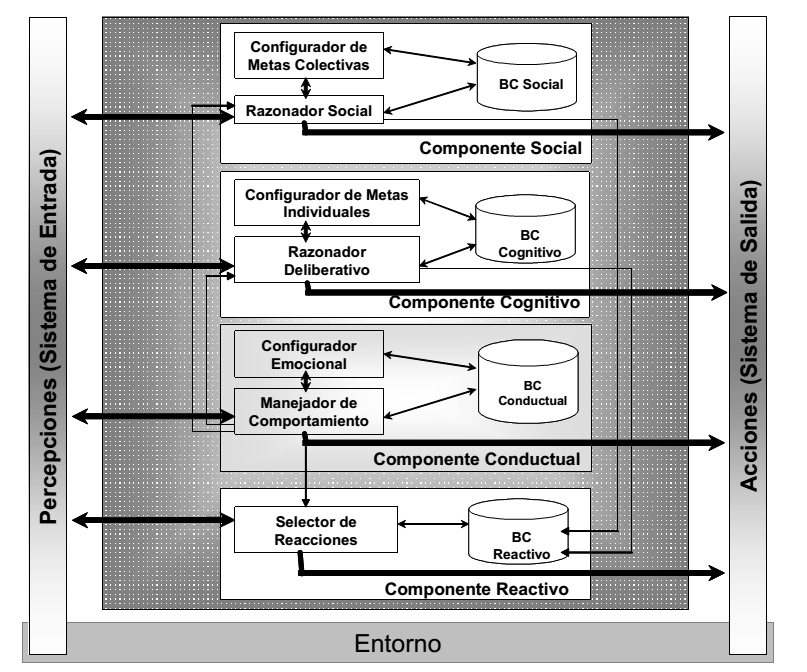
\includegraphics[width=6cm]{ilustraciones/componentes-masoes-individual}
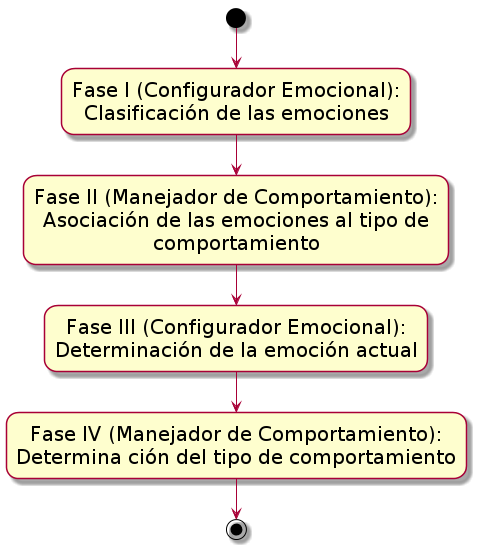
\includegraphics[width=4cm]{ilustraciones/componente-conductual}
\end{frame}

\begin{frame}
\frametitle{MASOES}
\framesubtitle{Modelo Afectivo de MASOES}
\centering
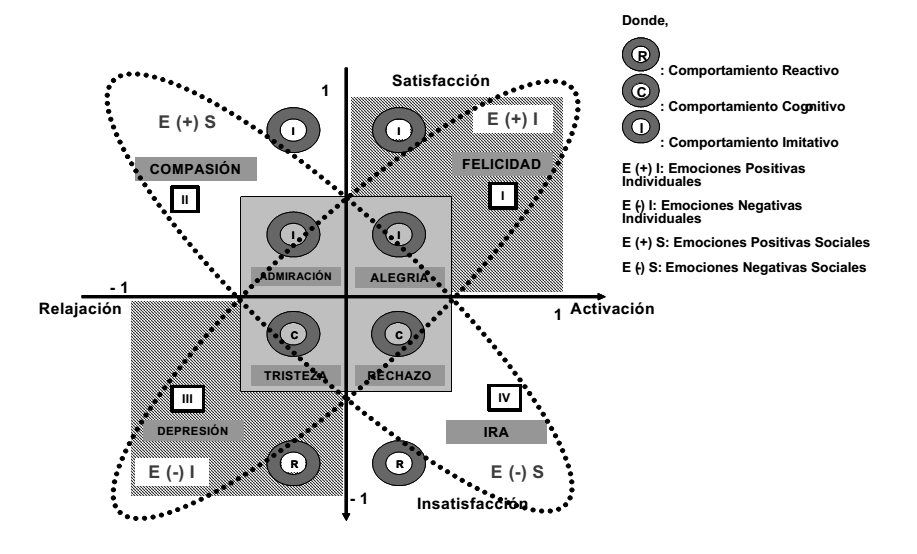
\includegraphics[width=7cm]{ilustraciones/modelo-afectivo}
\end{frame}

\begin{frame}
\frametitle{MASOES}
\framesubtitle{Reglas de Priorización de Comportamientos}
\begin{table}[!ht]
\centering
\scriptsize
\begin{tabular}{ll}
\hline
\textbf{Regla 1:} & Si el \textit{Estado Emocional} es \textit{Positivo} \\
& entonces priorizar \textit{Comportamiento Imitativo} \\
\textbf{Regla 2:} & Sino Si el \textit{Estado Emocional} es \textit{Ligeramente Negativo} \\
& entonces priorizar \textit{Comportamiento Cognitivo} \\
\textbf{Regla 3:} & Sino Si el \textit{Estado Emocional} es \textit{Altamente Negativo} \\
& entonces priorizar \textit{Comportamiento Reactivo} \\
\hline
\end{tabular}
\end{table}
\end{frame}

\section{Propuesta}

\begin{frame}
\frametitle{Propuesta}
\framesubtitle{Aspectos Arquitecturales}
\begin{columns}
\column{0.5\textwidth}
\textbf{JADE}\\
\textbf{Java Agent
DEvelopment}, uno de los marcos de trabajo con paradigma de POA (\textbf{Programación Orientada a Agentes})
más populares, implementado en el lenguaje de programación Java
\column{0.5\textwidth}
\textbf{FIPA}\\
\textbf{Foundation for Intelligent Physical Agents},
las cuales representan una colección de normas que tienen como objetivo promover la interoperabilidad
de agentes heterogéneos y los servicios que pueden representar
\end{columns}
\end{frame}

\begin{frame}
\frametitle{Propuesta}
\framesubtitle{Aspectos Arquitecturales}
\centering
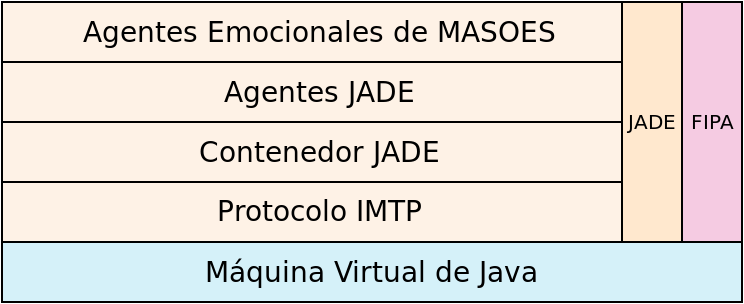
\includegraphics[width=6cm]{ilustraciones/arquitectura}
\vfill
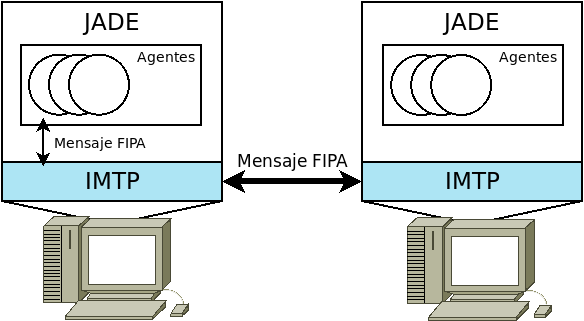
\includegraphics[width=6cm]{ilustraciones/comunicacion-entre-hosts}
\end{frame}

\begin{frame}
\frametitle{Aspectos Propuestos a Nivel Individual}
\framesubtitle{Propuesta de Una Ontología Para MASOES}
\begin{columns}
\column{0.5\textwidth}
\centering
\tiny
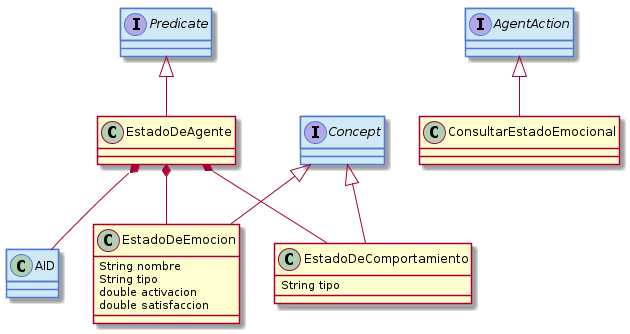
\includegraphics[width=5cm]{ilustraciones/ontologia-masoes-estado}
\\
Acción Consultar Estado del Agente
\column{0.5\textwidth}
\centering
\tiny
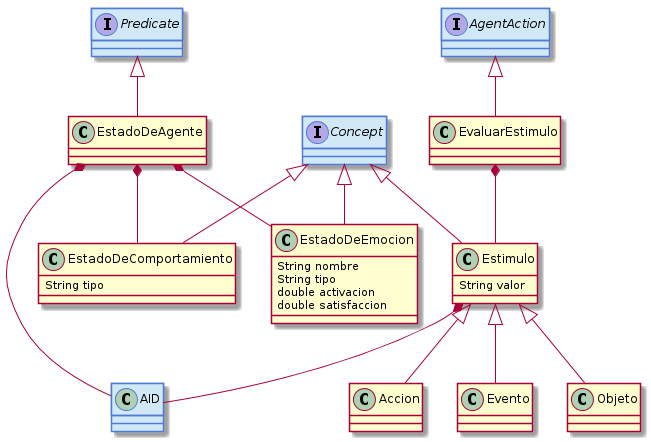
\includegraphics[width=5cm]{ilustraciones/ontologia-masoes-estimulo}
\\
Acción Evaluar Estímulo
\end{columns}
\end{frame}

\begin{frame}
\frametitle{Aspectos Propuestos a Nivel Individual}
\framesubtitle{Diseño del Agente Emocional}
\centering
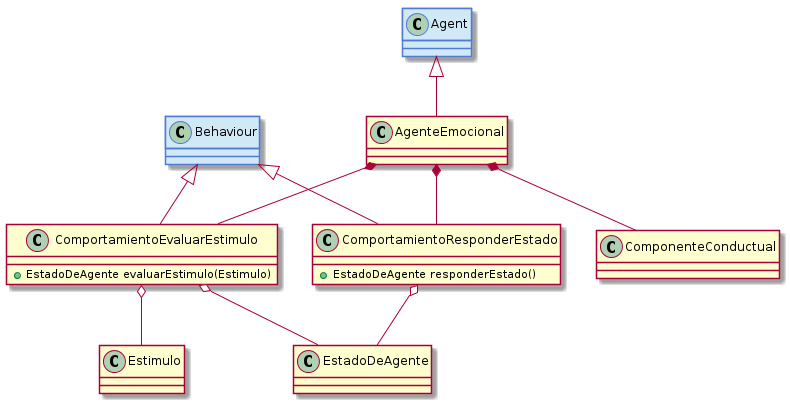
\includegraphics[width=7cm]{ilustraciones/diseno-nivel-individual}
\end{frame}

\begin{frame}
\frametitle{Aspectos Propuestos a Nivel Individual}
\framesubtitle{Diseño del Componente Conductual}
\centering
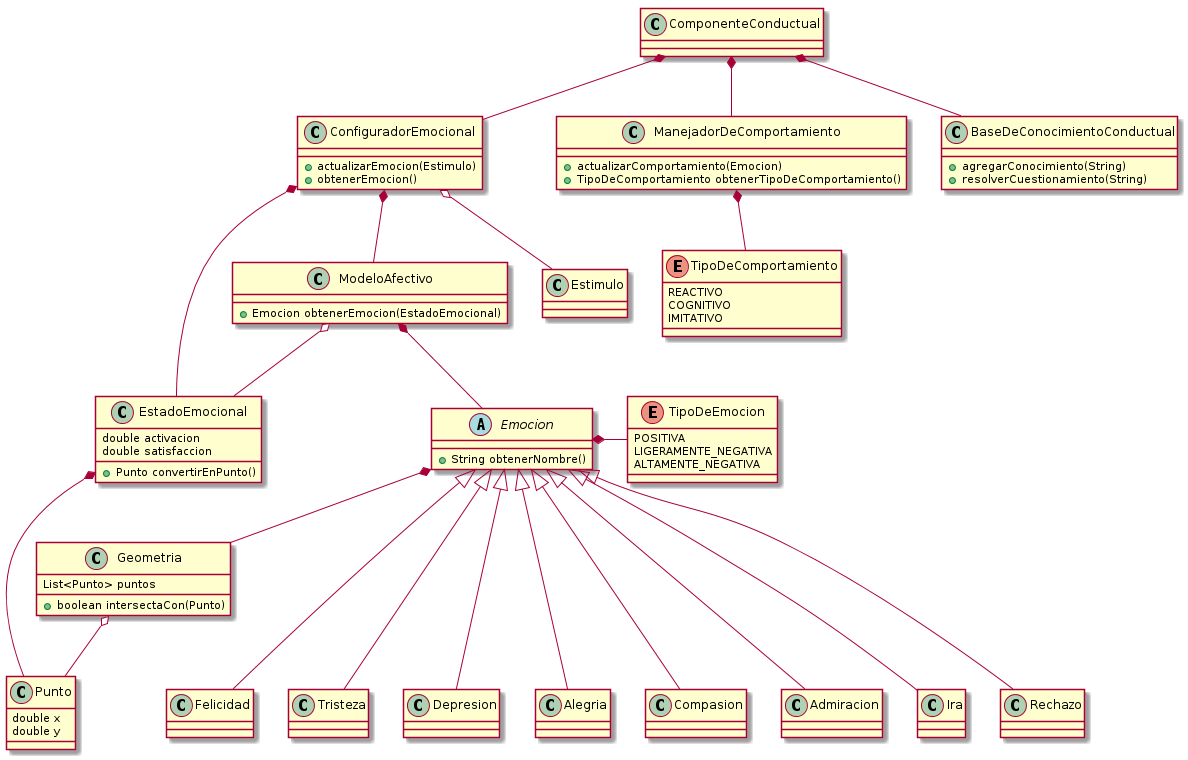
\includegraphics[width=9cm]{ilustraciones/diseno-componente-conductual}
\end{frame}

\begin{frame}
\frametitle{Componente Conductual}
\framesubtitle{Procesamiento de Estímulo}
\centering
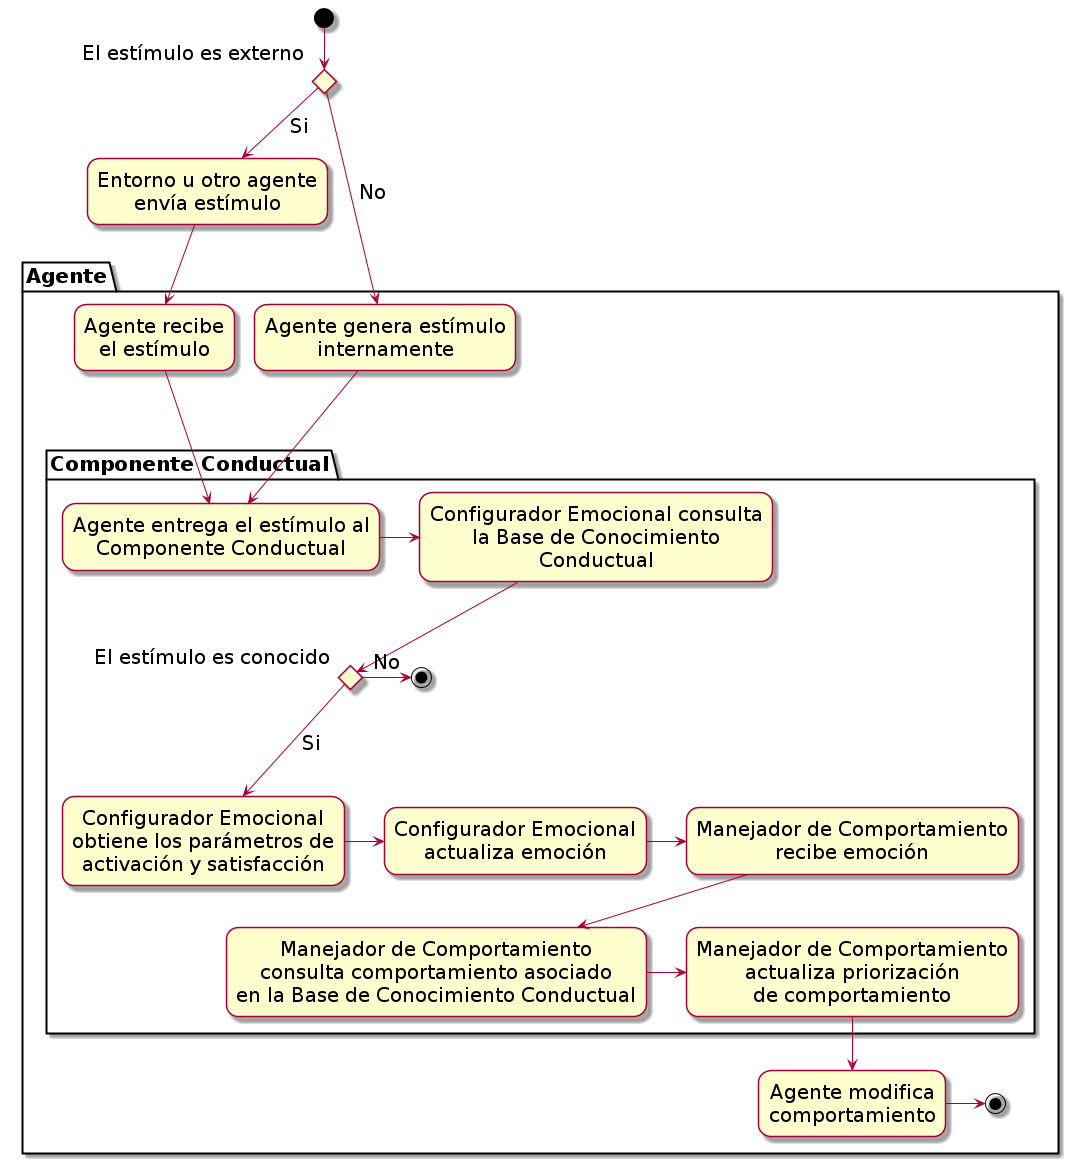
\includegraphics[width=6cm]{ilustraciones/procesamiento-estimulo}
\end{frame}

\begin{frame}
\frametitle{Aspectos Propuestos a Nivel Colectivo}
\framesubtitle{Calculo de la Emoción Social}
\begin{exampleblock}{Emoción Social}
$ES(Ag) = \{EC(Ag), m(Ag), \sigma(Ag)\}$
\end{exampleblock}

Donde $Ag$ representa al grupo de agentes en estudio, $EC(Ag)$ se refiere a la
emoción central exhibida por el grupo de agentes, $m(Ag)$ es el estado emocional
más alejado de la $EC$, $\sigma(Ag)$ representa la dispersión emocional entorno
a la $EC$.
\end{frame}

\begin{frame}
\frametitle{Aspectos Propuestos a Nivel Colectivo}
\framesubtitle{Calculo de la Emoción Social}
\begin{exampleblock}{Emoción Central}
$EC(Ag) = (\bar A(Ag), \bar S(Ag))$
\end{exampleblock}

\begin{exampleblock}{Promedio de la Activación}
$\bar A(Ag)=\frac{\sum_{i=1}^n A_i}{n}, \forall ag_i \in Ag$ \\
\end{exampleblock}

\begin{exampleblock}{Promedio de la Satisfacción}
$\bar S(Ag)=\frac{\sum_{i=1}^n S_i}{n}, \forall ag_i \in Ag$
\end{exampleblock}

\end{frame}

\begin{frame}
\frametitle{Aspectos Propuestos a Nivel Colectivo}
\framesubtitle{Calculo de la Emoción Social}
\begin{exampleblock}{Distancia Máxima}
$ m(Ag) = (m_A(Ag), m_S(Ag))$
\end{exampleblock}

\begin{exampleblock}{Distancia Máxima de la Activación}
$m_A(Ag) = max\left(\sqrt{(A_i - \bar A(Ag))^2}\right), \forall ag_i \in Ag$
\end{exampleblock}

\begin{exampleblock}{Distancia Máxima de la Satisfacción}
$m_S(Ag) = max\left(\sqrt{(S_i - \bar S(Ag))^2}\right), \forall ag_i \in Ag$
\end{exampleblock}

\end{frame}

\begin{frame}
\frametitle{Aspectos Propuestos a Nivel Colectivo}
\framesubtitle{Calculo de la Emoción Social}
\begin{exampleblock}{Dispersión Emocional}
$ \sigma(Ag) = (\sigma_A(Ag), \sigma_S(Ag))$
\end{exampleblock}

\begin{exampleblock}{Dispersión Emocional de la Activación}
$\sigma_A(Ag) = \sqrt{\frac{\sum_{i=1}^n(A_i - \bar A(Ag))^2}{n}},  \forall ag_i \in Ag$
\end{exampleblock}

\begin{exampleblock}{Dispersión Emocional de la Satisfacción}
$  \sigma_S(Ag) = \sqrt{\frac{\sum_{i=1}^n(S_i - \bar S(Ag))^2}{n}},  \forall ag_i \in Ag$
\end{exampleblock}
\end{frame}

\section{Casos de Estudio}
\begin{frame}
\frametitle{Casos de Estudio}

\end{frame}

\DoBlueBackgroundTitle{Demostración}

\section{Conclusión}
\begin{frame}
\frametitle{Conclusión}

\end{frame}

\DoBlueBackgroundTitle{Preguntas}

\ThankYouFrame

\end{document}
